\begin{figure}[!ht]
    \centering
    \setlength{\resLen}{2.1in}
    \addtolength{\tabcolsep}{-5.5pt}
    \small
    \begin{tabular}{ccc|ccc|ccc}
        \multicolumn{3}{c}{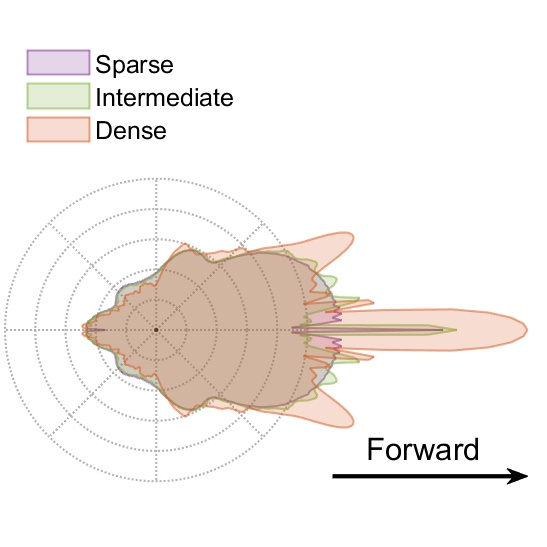
\includegraphics[width=\resLen]{waveoptics/pfunc/distance.jpg}} &
        \multicolumn{3}{c}{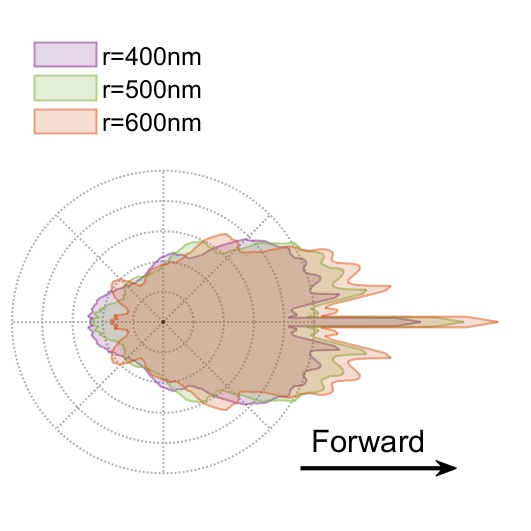
\includegraphics[width=\resLen]{waveoptics/pfunc/radius.jpg}} &
        \multicolumn{3}{c}{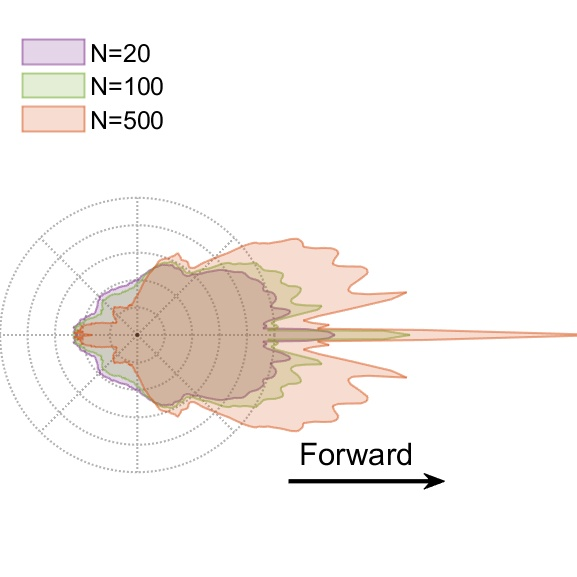
\includegraphics[width=\resLen]{waveoptics/pfunc/number.jpg}} \\[-5pt]
        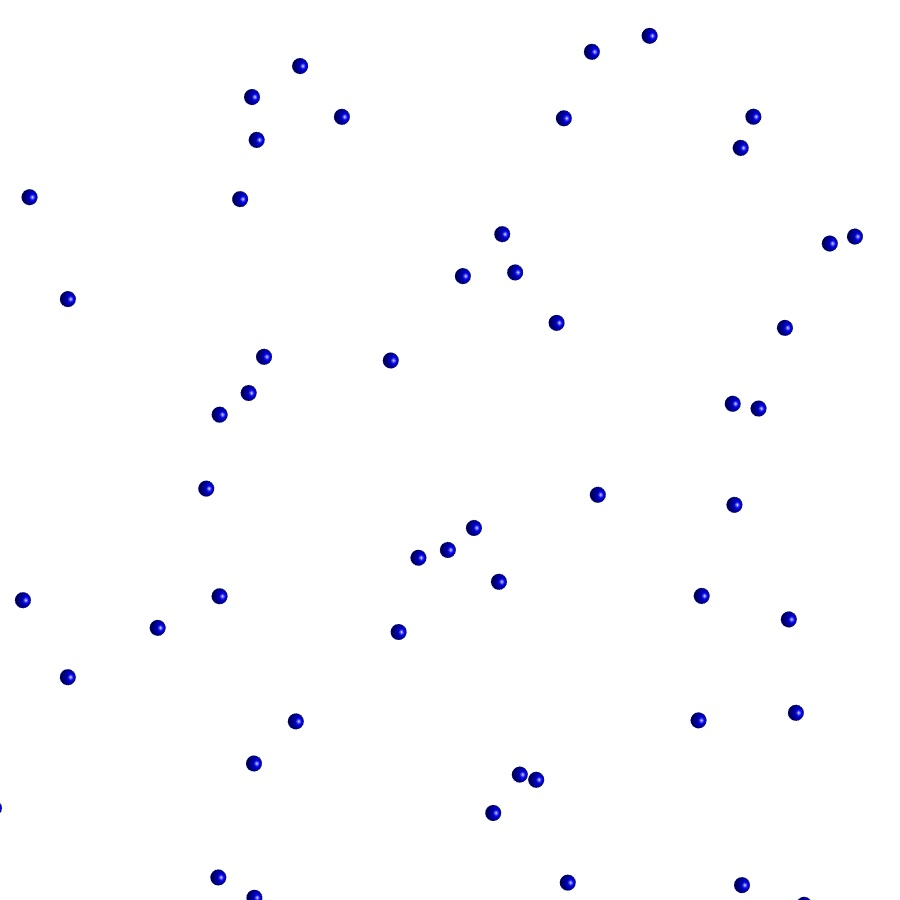
\includegraphics[width=0.33\resLen]{waveoptics/particle/validate2_D1_N100_500nm.jpg} &
        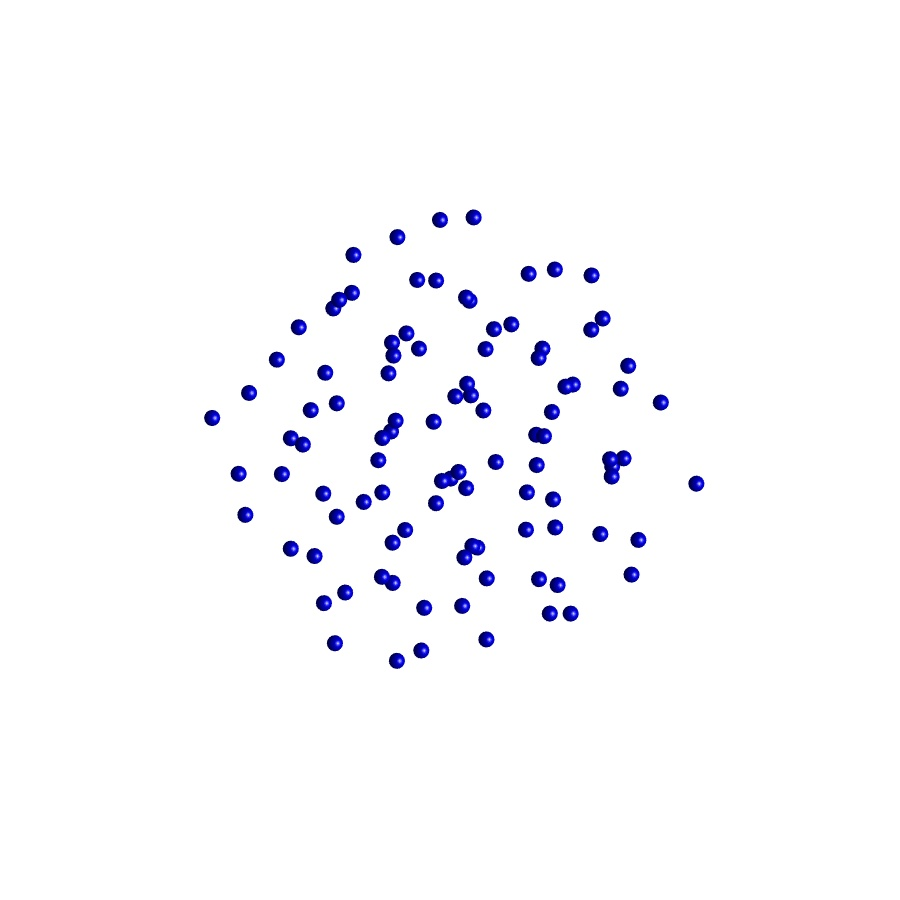
\includegraphics[width=0.33\resLen]{waveoptics/particle/validate3_D2_N100_500nm.jpg} &
        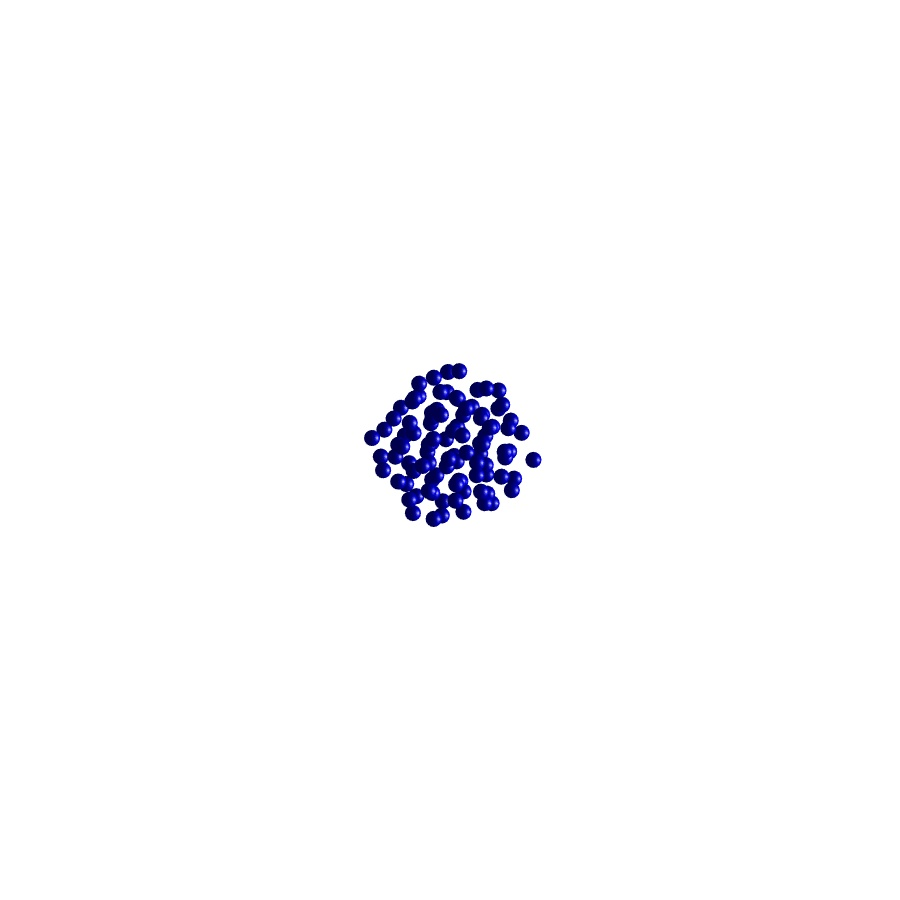
\includegraphics[width=0.33\resLen]{waveoptics/particle/validate4_D3_N100_500nm.jpg} &
        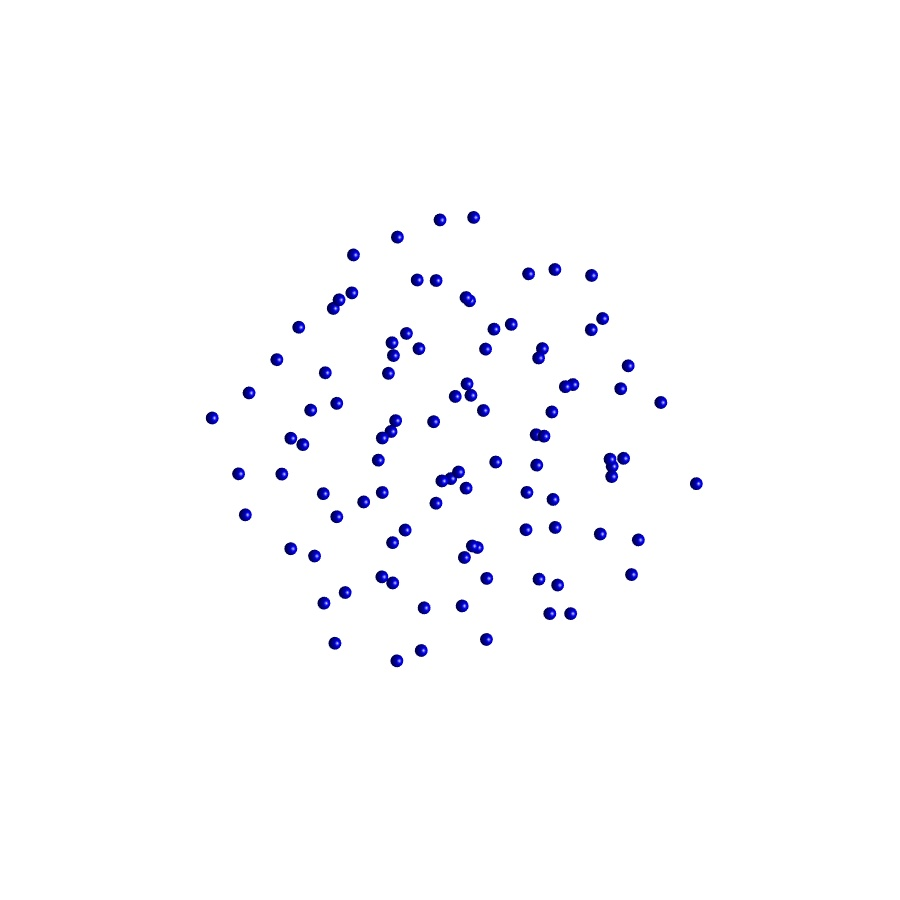
\includegraphics[width=0.33\resLen]{waveoptics/particle/validate5_D2_N100_400nm.jpg} &
        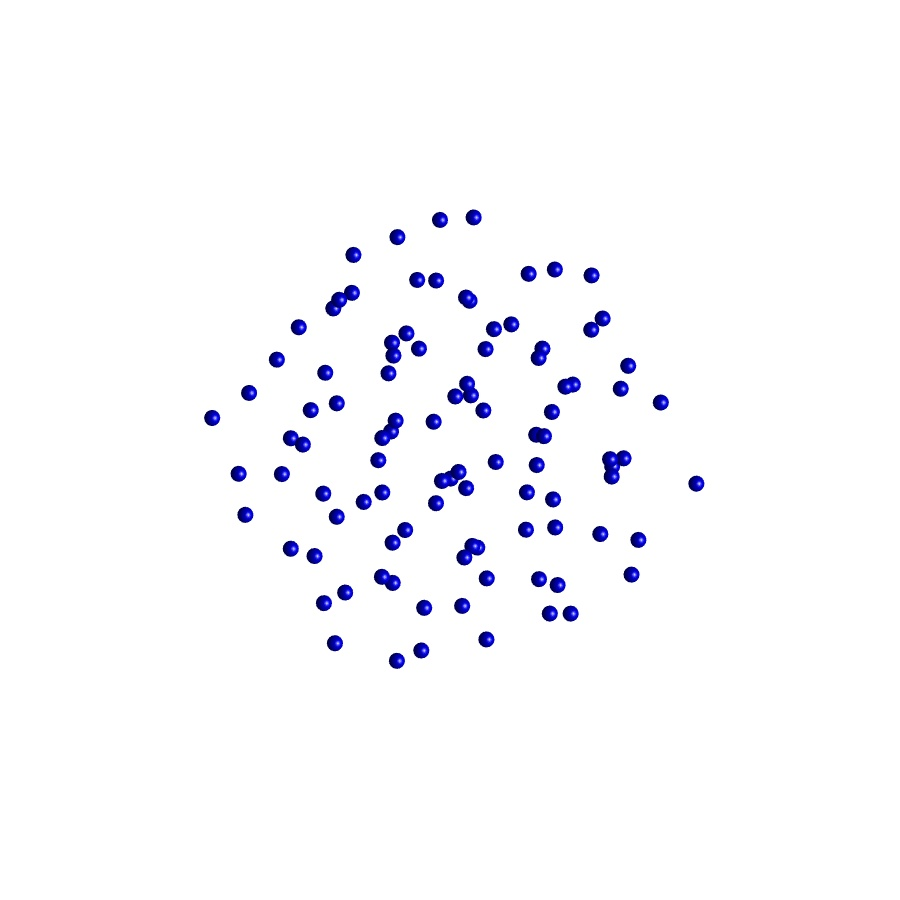
\includegraphics[width=0.33\resLen]{waveoptics/particle/validate3_D2_N100_500nm.jpg} &
        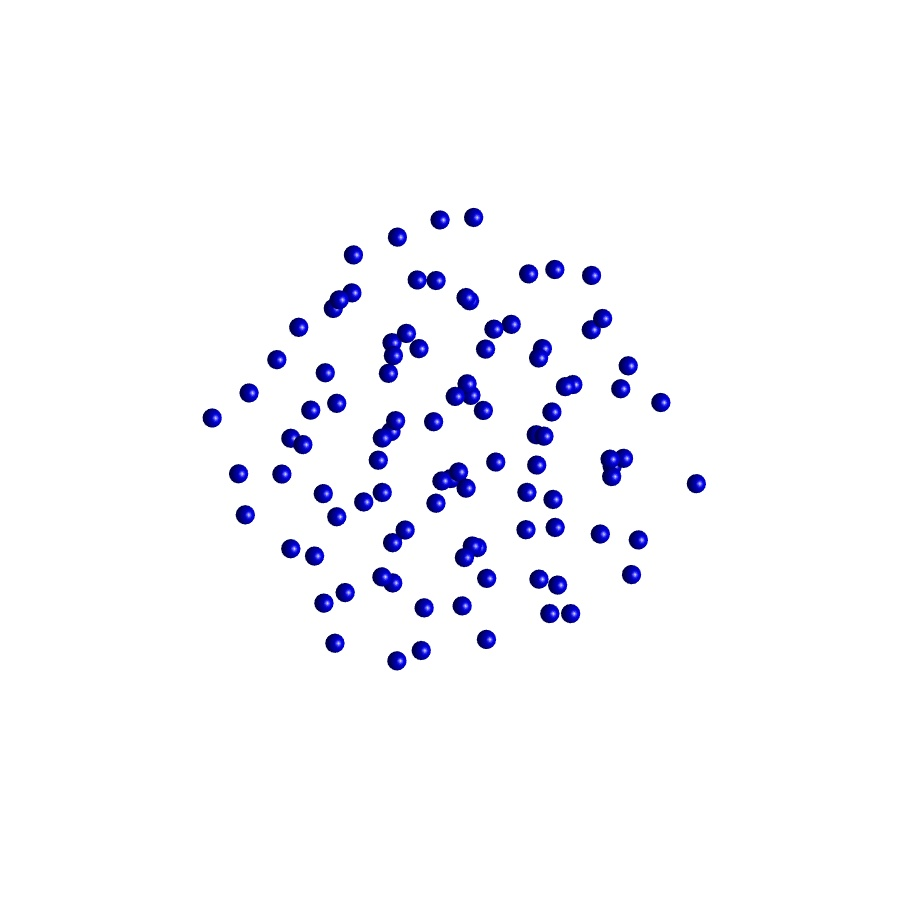
\includegraphics[width=0.33\resLen]{waveoptics/particle/validate7_D2_N100_600nm.jpg} &
        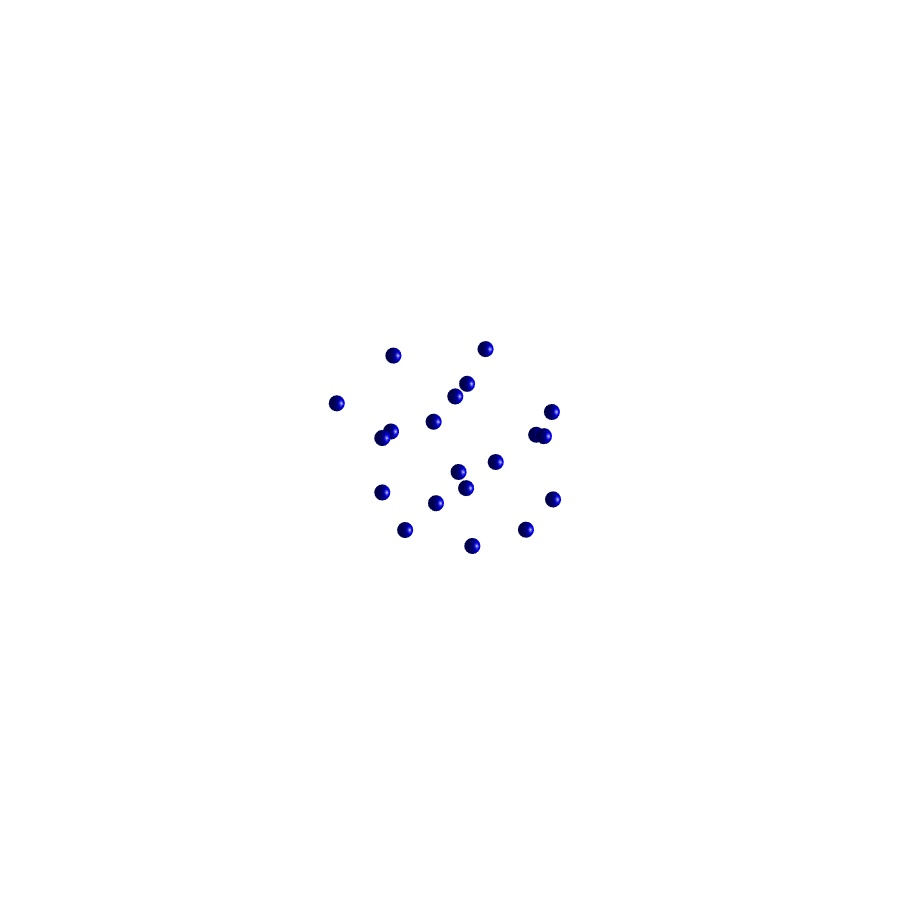
\includegraphics[width=0.33\resLen]{waveoptics/particle/validate8_D2_N20_500nm.jpg} &
        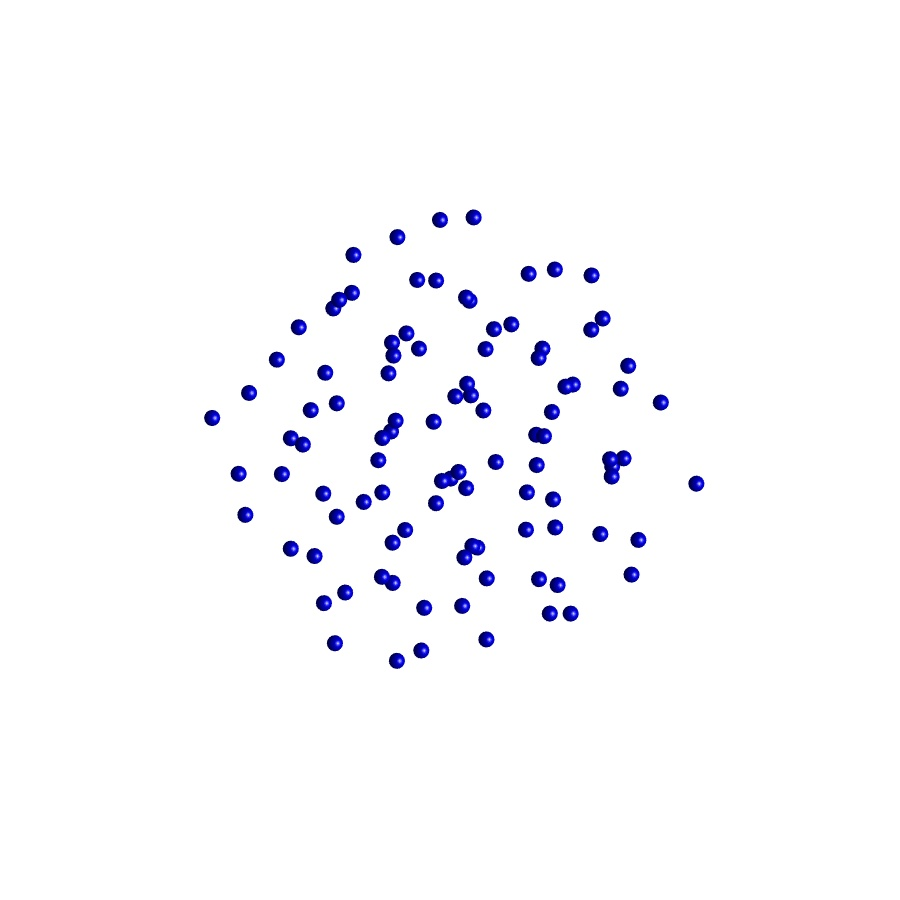
\includegraphics[width=0.33\resLen]{waveoptics/particle/validate3_D2_N100_500nm.jpg} &
        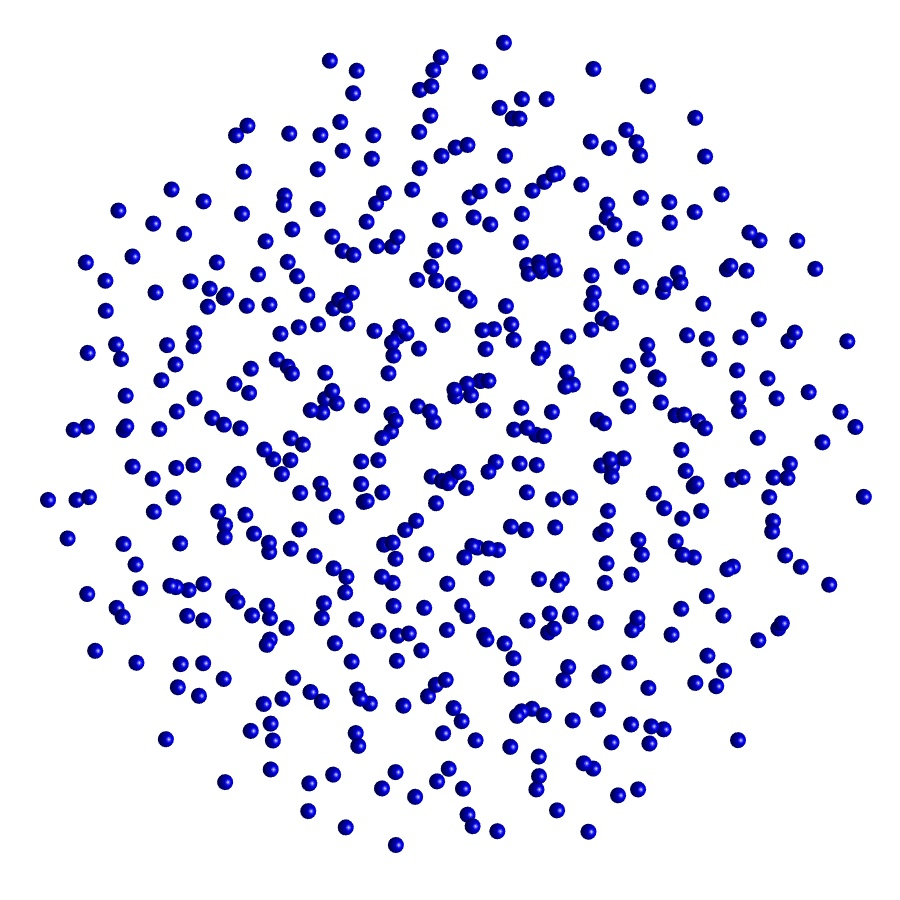
\includegraphics[width=0.33\resLen]{waveoptics/particle/validate10_D2_N500_500nm.jpg} 
        \\
        Sparse & Intermediate & Dense & $a_i$=400nm & 500nm & 600nm &
        $\Ncls=20$ & $100$ & $500$ \\ [5pt]
        \multicolumn{3}{c}{\textbf{(a)} Varying particles spacing} &
        \multicolumn{3}{c}{\textbf{(b)} Varying particles radius} &
        \multicolumn{3}{c}{\textbf{(c)} Varying particles count} 
    \end{tabular}
    \caption[Comparison for different parameters]{\label{fig:waveoptics:ablation}
        \textbf{Comparison of the resulting phase function} for different cluster parameters, for a planar incident field at $\lambda=700$nm. Unless mentioned otherwise, the clusters have $\Ncls=100$ particles, and each particle has radius $a_i=500$nm. For each phase function, we vary: (a) The distance between particles within the cluster; (b) The particle size $a_i$; and (c) The number of particles $\Ncls$. 
    }
\end{figure}